\documentclass[12pt,a4paper]{article}

% ─── 1. PACKAGES ──────────────────────────────────────────────────────────────
\usepackage[utf8]{inputenc}
\usepackage[T1]{fontenc}
\usepackage{amsmath, amssymb}
\usepackage{geometry}
\usepackage{graphicx}
\usepackage{xcolor}
\usepackage{listings}
\usepackage{hyperref}
\usepackage{booktabs}
\usepackage{enumitem}
\usepackage{tcolorbox}
\usepackage{mdframed}
\usepackage{fancyhdr}
\usepackage{titlesec}
\usepackage{tikz} % Untuk menggambar diagram state NFA
\usetikzlibrary{automata, positioning, arrows.meta}

% Font Settings
\usepackage{newtxtext,newtxmath} % Times New Roman
\usepackage{courier}             % Courier New untuk kode

\geometry{margin=2.5cm}

% ─── 2. WARNA TEMA ────────────────────────────────────────────────────────────
\definecolor{codebg}{RGB}{245,247,250}
\definecolor{codeframe}{RGB}{180,195,215}
\definecolor{keywordcolor}{RGB}{0,112,192}
\definecolor{commentcolor}{RGB}{100,160,100}
\definecolor{stringcolor}{RGB}{180,70,50}
\definecolor{notebg}{RGB}{255,249,230}
\definecolor{noteframe}{RGB}{230,180,50}
\definecolor{tipbg}{RGB}{230,245,235}
\definecolor{tipframe}{RGB}{50,160,90}
\definecolor{sectioncolor}{RGB}{30,80,150}

% ─── 3. STYLE SECTION & TOC ───────────────────────────────────────────────────
\titleformat{\section}{\Large\bfseries\color{sectioncolor}}{}{0em}{\thesection\quad}[\titlerule]
\titleformat{\subsection}{\large\bfseries\color{sectioncolor!80}}{}{0em}{\thesubsection\quad}

% Style Table of Contents
\usepackage{tocloft}
\renewcommand{\cftsecleader}{\cftdotfill{\cftdotsep}}
\renewcommand{\cftsecfont}{\bfseries\color{sectioncolor}}

% ─── 4. LISTINGS (CODE STYLE) ─────────────────────────────────────────────────
\lstdefinestyle{customstyle}{
  basicstyle=\ttfamily\small,
  backgroundcolor=\color{codebg},
  frame=single,
  rulecolor=\color{codeframe},
  keywordstyle=\bfseries\color{keywordcolor},
  commentstyle=\itshape\color{commentcolor},
  stringstyle=\color{stringcolor},
  numbers=left,
  numberstyle=\tiny\color{gray},
  breaklines=true,
  tabsize=4,
  showstringspaces=false
}
\lstset{style=customstyle}

% ─── 5. KOTAK CATATAN (MD-FRAME) ──────────────────────────────────────────────
\newmdenv[
  backgroundcolor=notebg, linecolor=noteframe, linewidth=2pt,
  leftline=true, topline=false, rightline=false, bottomline=false,
  innerleftmargin=10pt, innertopmargin=6pt, innerbottommargin=6pt, skipabove=8pt
]{notebox}

\newmdenv[
  backgroundcolor=tipbg, linecolor=tipframe, linewidth=2pt,
  leftline=true, topline=false, rightline=false, bottomline=false,
  innerleftmargin=10pt, innertopmargin=6pt, innerbottommargin=6pt, skipabove=8pt
]{tipbox}

% ─── 6. HEADER & FOOTER ───────────────────────────────────────────────────────
\pagestyle{fancy}
\fancyhf{}
\fancyhead[L]{\small\textit{Teori Bahasa dan Automata}}
\fancyhead[R]{\small\textit{Modul Pembelajaran -- NFA}}
\fancyfoot[C]{\thepage}
\renewcommand{\headrulewidth}{0.4pt}

% ─── 7. DATA COVER ────────────────────────────────────────────────────────────
\title{
  {\LARGE\bfseries TEORI BAHASA DAN AUTOMATA}\\[0.5em]
  {\large Modul Pembelajaran: Non-Deterministic Finite Automata (NFA)}\\[0.8em]
  {\normalsize Penjelasan mendalam mengenai konsep non-determinisme, transisi epsilon ($\epsilon$), definisi matematis, dan studi kasus perancangan mesin NFA.}
}
\author{}
\date{}

% ==============================================================================
\begin{document}

\maketitle
\thispagestyle{fancy}
\tableofcontents
\newpage

% ─── KONTEN MATERI ─────────────────────────────────────────────────────────────

\section{Mengenal Non-Deterministic Finite Automata (NFA)}

\subsection{Apa itu Mesin NFA dan Bedanya dengan DFA?}
Kalau sebelumnya kita udah belajar DFA yang sifatnya serba pasti dan kaku banget, sekarang kita kenalan sama saudaranya yang jauh lebih fleksibel, yaitu \textit{Non-Deterministic Finite Automaton} (NFA). Secara fisik bayangannya mirip: ada mesin, ada pita input (\textit{Input Tape}), dan head yang ngebaca karakter satu per satu dari kiri ke kanan.

Tapi, \textbf{cara kerjanya beda banget}. Sifat "Non-Deterministik" di sini bikin mesin NFA punya kemampuan buat "menebak" atau bercabang. Di NFA, kalau mesin dapet satu input, dia nggak cuma punya satu jalan pasti. Dia bisa bereaksi dengan tiga cara ini:
\begin{itemize}
    \item \textbf{Bercabang (Multiple Paths):} Satu karakter input bisa bikin mesin loncat ke lebih dari satu \textit{state} sekaligus.
    \item \textbf{Jalan Buntu (Dead End):} Mesin bisa aja nggak punya jalur panah transisi buat suatu karakter tertentu. Kalau dapet karakter itu, cabangnya langsung mati (gagal).
    \item \textbf{Gerak Gaib (Epsilon Transition):} Mesin bisa loncat ke \textit{state} lain secara tiba-tiba tanpa perlu ngebaca karakter apa pun dari pita! Ini yang paling sakti di NFA.
\end{itemize}

\begin{notebox}
\textbf{Analogi Sederhana NFA} \\
Bayangin NFA ini kayak kamu lagi main game yang ada jalan bercabang. Tiap ketemu persimpangan, karakter kamu bakal "ngekloning" dirinya sendiri dan nyusurin semua jalan yang ada secara bersamaan. Kalau salah satu aja dari kloningan itu nyampe ke garis finish (\textit{Final State}) pas waktu habis, kamu menang (\textit{Accept}). Kloningan lain yang nyasar atau mati di jalan buntu nggak bakal ngaruh selama ada satu yang sukses.
\end{notebox}

\subsection{Syarat Diterimanya String di NFA}
Karena mesinnya jalan bercabang secara paralel, aturan main diterimanya string jadi lebih longgar dibandingkan DFA.
\begin{itemize}
    \item \textbf{Diterima (Accept):} String diterima kalau ada \textbf{setidaknya satu} jalur komputasi (salah satu kloningan) yang berhasil berhenti pas di \textit{Final State} setelah karakter terakhir dibaca.
    \item \textbf{Ditolak (Reject):} String cuma bakal ditolak kalau \textbf{semua} jalur yang dicoba ternyata jalan buntu, atau ujung-ujungnya berakhir di \textit{state} biasa (bukan \textit{Final State}).
\end{itemize}

\newpage
\section{Transisi Kosong: Epsilon ($\epsilon$)}

Ini adalah salah satu fitur paling unik dari NFA yang sering banget dipakai, yaitu Transisi Epsilon ($\epsilon$-transition). Di beberapa buku teks, kadang ditulis pakai lambda ($\lambda$), tapi maksudnya sama aja.

\subsection{Gimana Cara Kerja Transisi Epsilon?}
Biasanya, buat pindah dari \textit{state} A ke \textit{state} B, mesin butuh "ongkos" berupa membaca satu karakter dari pita input. Nah, panah yang dilabeli $\epsilon$ ini artinya jalan tol gratis. Mesin boleh pindah ke state tujuan tanpa perlu mengonsumsi atau membaca karakter dari pita sama sekali.

\begin{figure}[h]
    \centering
    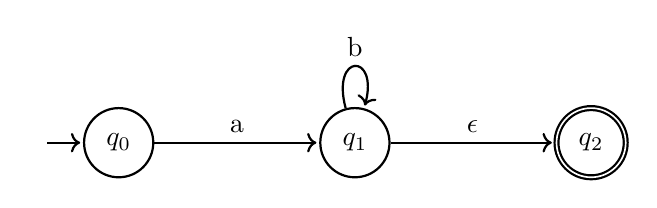
\begin{tikzpicture}[shorten >=1pt,node distance=3cm,on grid,auto, thick]
       \node[state,initial,initial text=] (q0) {$q_0$};
       \node[state] (q1) [right=of q0] {$q_1$};
       \node[state,accepting] (q2) [right=of q1] {$q_2$};

       \path[->] 
       (q0) edge node {a} (q1)
       (q1) edge node {$\epsilon$} (q2)
            edge [loop above] node {b} (q1);
    \end{tikzpicture}
    \caption{Contoh Transisi Epsilon. Dari $q_1$, mesin bisa seketika berada di $q_2$ tanpa baca huruf apa pun.}
\end{figure}

Fitur ini ngebantu banget pas kita mau merancang mesin untuk mendeteksi berbagai pola bahasa yang kompleks, karena kita bisa menghubungkan berbagai mesin kecil jadi satu kesatuan dengan gampang pakai jalan tol $\epsilon$ ini.

\newpage
\section{Definisi Formal dan Tabel Transisi NFA}

Sama kayak DFA, NFA juga digambarkan pakai model matematika 5-tupel: $M = (Q, \Sigma, \delta, q_0, F)$. Bedanya cuma ada di satu tempat, yaitu di **Fungsi Transisinya ($\delta$)**.

\begin{itemize}
    \item \textbf{$Q$}: Himpunan semua \textit{state}.
    \item \textbf{$\Sigma$}: Himpunan alfabet (karakter input). Tapi ingat, $\epsilon$ bukan bagian dari alfabet input ya!
    \item \textbf{$q_0$}: \textit{State} awal.
    \item \textbf{$F$}: Himpunan \textit{Final State}.
    \item \textbf{$\delta$ (Fungsi Transisi)}: Nah ini bedanya. Di NFA, pemetaannya adalah $\delta : Q \times (\Sigma \cup \{\epsilon\}) \rightarrow \mathcal{P}(Q)$. 
\end{itemize}

Maksud dari $\mathcal{P}(Q)$ (Powerset / Himpunan Kuasa) itu apa? Artinya, hasil dari fungsi transisi NFA \textbf{bukanlah satu state tunggal}, melainkan \textbf{sebuah himpunan} state. Himpunan ini bisa isinya satu state, bisa isinya banyak state, atau bahkan bisa himpunan kosong ($\emptyset$) kalau ternyata jalannya buntu.

\subsection{Tabel Transisi NFA}
Karena hasil pemetaannya berupa himpunan, cara nulis di tabel transisinya juga harus pakai kurung kurawal \{\}.

Misal kita punya NFA di mana di state $q_0$ baca '0' bisa ke $q_0$ atau ke $q_1$, baca '1' cuma ke $q_0$, dan ada transisi $\epsilon$ dari $q_1$ ke $q_2$.

\begin{table}[h]
\centering
\begin{tabular}{@{}cccc@{}}
\toprule
\textbf{$\delta$} & \textbf{0} & \textbf{1} & \textbf{$\epsilon$} \\ \midrule
$\rightarrow q_0$ & $\{q_0, q_1\}$ & $\{q_0\}$ & $\emptyset$ \\
$q_1$ & $\emptyset$ & $\emptyset$ & $\{q_2\}$ \\
$*q_2$ & $\emptyset$ & $\emptyset$ & $\emptyset$ \\ \bottomrule
\end{tabular}
\caption{Tabel Transisi NFA. Perhatikan pemakaian kurung kurawal dan himpunan kosong ($\emptyset$).}
\end{table}

\newpage
\section{Kumpulan Studi Kasus Perancangan NFA}

Merancang NFA itu rasanya jauh lebih gampang dan lebih natural dibanding ngerancang DFA. Kenapa? Karena kita tinggal fokus bikin jalur buat string yang bener aja. Kalau buat string yang salah, gampang, biarin aja buntu!

\subsection{Kasus 1: Pola Berakhiran "01"}
Kita pengen bikin mesin buat bahasa $L = \{w \mid w \text{ diakhiri dengan } 01\}$. Karakter apa pun di depannya bebas.

Kalau pakai DFA, ini bakal lumayan mikir karena harus bikin \textit{loop back} kalau polanya gagal di tengah jalan. Tapi kalau pakai NFA, desainnya \textit{straightforward} banget!

\begin{figure}[h]
    \centering
    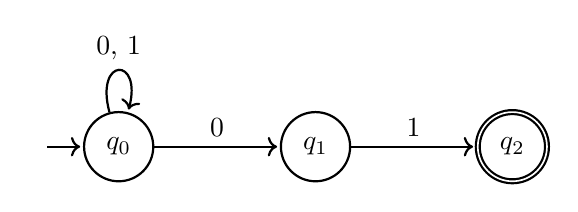
\begin{tikzpicture}[shorten >=1pt,node distance=2.5cm,on grid,auto, thick]
       \node[state,initial,initial text=] (q0) {$q_0$};
       \node[state] (q1) [right=of q0] {$q_1$};
       \node[state,accepting] (q2) [right=of q1] {$q_2$};

       \path[->] 
       (q0) edge [loop above] node {0, 1} (q0)
            edge node {0} (q1)
       (q1) edge node {1} (q2);
    \end{tikzpicture}
    \caption{NFA String Berakhiran "01"}
\end{figure}

\textbf{Bedah Alurnya (Misal input "1001"):}
\begin{itemize}
    \item Awal di $q_0$. Baca '1', cuma bisa ngeloop di $q_0$.
    \item Baca '0' pertama: mesin ngekloning diri. Satu tetap di $q_0$, satu lagi maju ke $q_1$.
    \item Baca '0' kedua: kloningan di $q_0$ ngekloning diri lagi (ada yang tetep di $q_0$, ada yang maju ke $q_1$). Kloningan yang tadi di $q_1$ malah \textbf{mati/buntu} karena di $q_1$ nggak ada panah buat huruf '0'.
    \item Baca '1' terakhir: kloningan yang ada di $q_1$ melesat ke $q_2$ (\textit{Final State}). Kloningan lain biarin aja terserah di mana. Karena ada satu yang nyampe di $q_2$, maka \textbf{Diterima}.
\end{itemize}

\subsection{Kasus 2: Mengandung Substring "11" atau "00"}
Gimana kalau kita mau deteksi string yang ada "11" berurutan ATAU "00" berurutan di dalamnya? Di sini transisi $\epsilon$ bakal sangat bersinar.

Kita pecah jadi tiga bagian:
1. Mesin tebakan awal (start).
2. Mesin pendeteksi "11".
3. Mesin pendeteksi "00".

\begin{figure}[h]
    \centering
    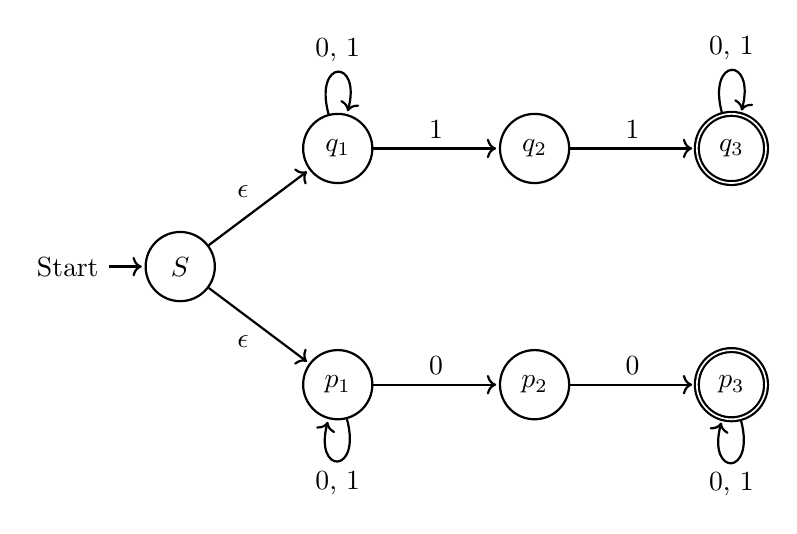
\begin{tikzpicture}[shorten >=1pt,node distance=2.5cm,on grid,auto, thick]
       \node[state,initial,initial text=Start] (S) {$S$};
       
       % Cabang atas untuk 11
       \node[state] (q1) [above right=1.5cm and 2cm of S] {$q_1$};
       \node[state] (q2) [right=of q1] {$q_2$};
       \node[state,accepting] (q3) [right=of q2] {$q_3$};

       % Cabang bawah untuk 00
       \node[state] (p1) [below right=1.5cm and 2cm of S] {$p_1$};
       \node[state] (p2) [right=of p1] {$p_2$};
       \node[state,accepting] (p3) [right=of p2] {$p_3$};

       \path[->] 
       (S) edge node [above left] {$\epsilon$} (q1)
           edge node [below left] {$\epsilon$} (p1)
           
       (q1) edge [loop above] node {0, 1} (q1)
            edge node {1} (q2)
       (q2) edge node {1} (q3)
       (q3) edge [loop above] node {0, 1} (q3)
       
       (p1) edge [loop below] node {0, 1} (p1)
            edge node {0} (p2)
       (p2) edge node {0} (p3)
       (p3) edge [loop below] node {0, 1} (p3);
    \end{tikzpicture}
    \caption{NFA dengan Transisi Epsilon mendeteksi "11" atau "00"}
\end{figure}

\textbf{Kenapa ini gampang banget dibikin?}
Pas mesin dinyalain, berkat transisi $\epsilon$, mesin seketika itu juga ngekloning dirinya sendiri tanpa baca apa-apa. Satu kloningan nangkring di $q_1$ buat nungguin dan nyari pola "11", sementara kloningan satunya lagi nangkring di $p_1$ buat nyari pola "00". Mereka kerja barengan secara paralel. Kalau salah satu dari pola itu ketemu duluan, beres! String langsung diterima. 

\subsection{Kasus 3: NFA Tanpa Jalan Buntu (Mirip DFA)}
Perlu diingat, setiap DFA itu adalah NFA, tapi nggak semua NFA itu DFA. NFA yang nggak pakai fitur \textit{multiple path} atau epsilon sama sekali, ya sebenarnya bentuknya persis kayak DFA. NFA cuma ngasih kita kebebasan: "Kamu boleh kok nggak nulis semua panahnya kalau emang nggak butuh." Kebebasan inilah yang bikin NFA jadi andalan pas kita mau ngedesain pola bahasa untuk tahap awal, sebelum nanti di- \textit{convert} jadi DFA buat urusan *coding* di program.

\end{document}